\documentclass[twocolumn, aps, apl]{revtex4-1}

\usepackage{graphicx}
\usepackage{fancyhdr}
\usepackage{amsmath}
\usepackage{caption}
\usepackage{enumerate}
\usepackage{subcaption}
\usepackage{textcomp}
\usepackage{placeins}
\usepackage{blindtext}

\begin{document}
\title{Lab 3. Low Noise Amplifiers }
\author{Albert Wandui}
\affiliation{EE 152: High Frequency Systems Lab.}
\maketitle

\section*{Introduction}\label{sec:introduction}
Talk about the steps involved in designing a good low noise amplifier.

\begin{itemize}
    \item talk about biasing briefly

    \item talk about stability and designing a good input matching network. Begin with a discussion on noise terms

    \item talk about designing the output matching network

    \item discuss the Y factor method used 

    \item discuss noise factors for the low pass filter as well as the amplifier in detail.
\end{itemize}

\section*{LNA Design}\label{sec:design}

\begin{itemize}
    \item selected the 2V 6 mA bias BJT because it had the lowest $T_{min} = 47.24 K$ at 4 GHz.

    \item made bias network, choosing $R_B = 45000 k \Omega$ and $R_c = 10 \Omega$. Placed large bias resistors close to $V_{cc}$ instead of next to the input of the transistor to prevent resonances between the resistor and the inductors in the network. Ideally should be placed close to minimize noise. See figure \ref{fig:dcnet}

    \begin{figure*}[!htbp]
        \centering
        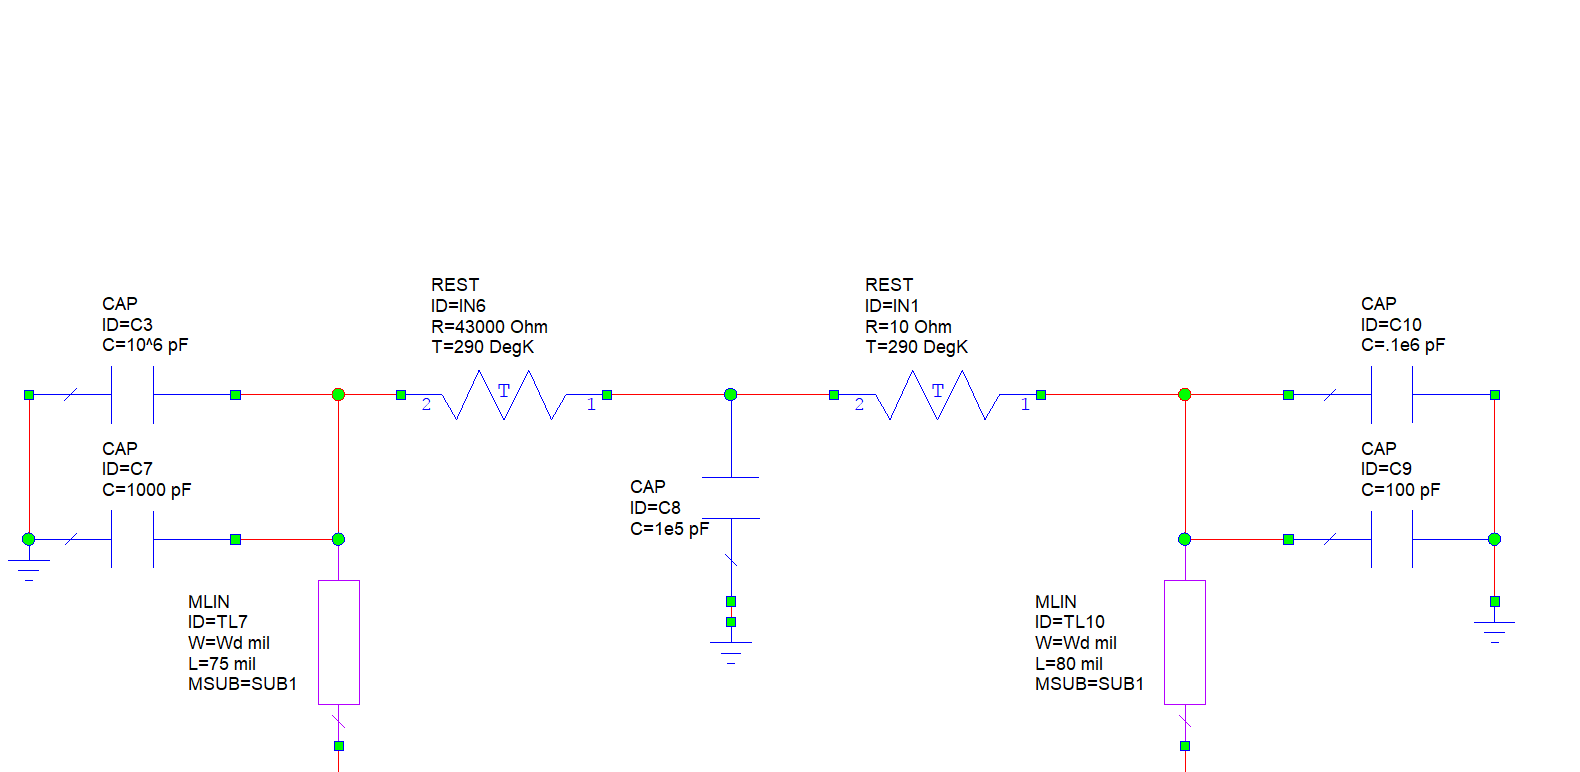
\includegraphics[scale=0.35]{dc_net.png}
        \caption{Schematic showing the bias resistors chosen to achieve a 6mA collector current and a 2V Bias in the design. The bypass capacitors are also shown.}
        \label{fig:dcnet}
    \end{figure*}

    \item changed all the microstrip widths to 21 mils and used the lengths specified in the diagram.

    \item added 5.6 nH inductors to the base and collector to improve stability. Using the .s2p files checked to ensure that there were no self-resonances in the region of interest. Had great stability above 2.5 GHz. See figure \ref{fig:LNAnet}, \ref{fig:stability}

    \begin{figure*}[!htbp]
        \centering
        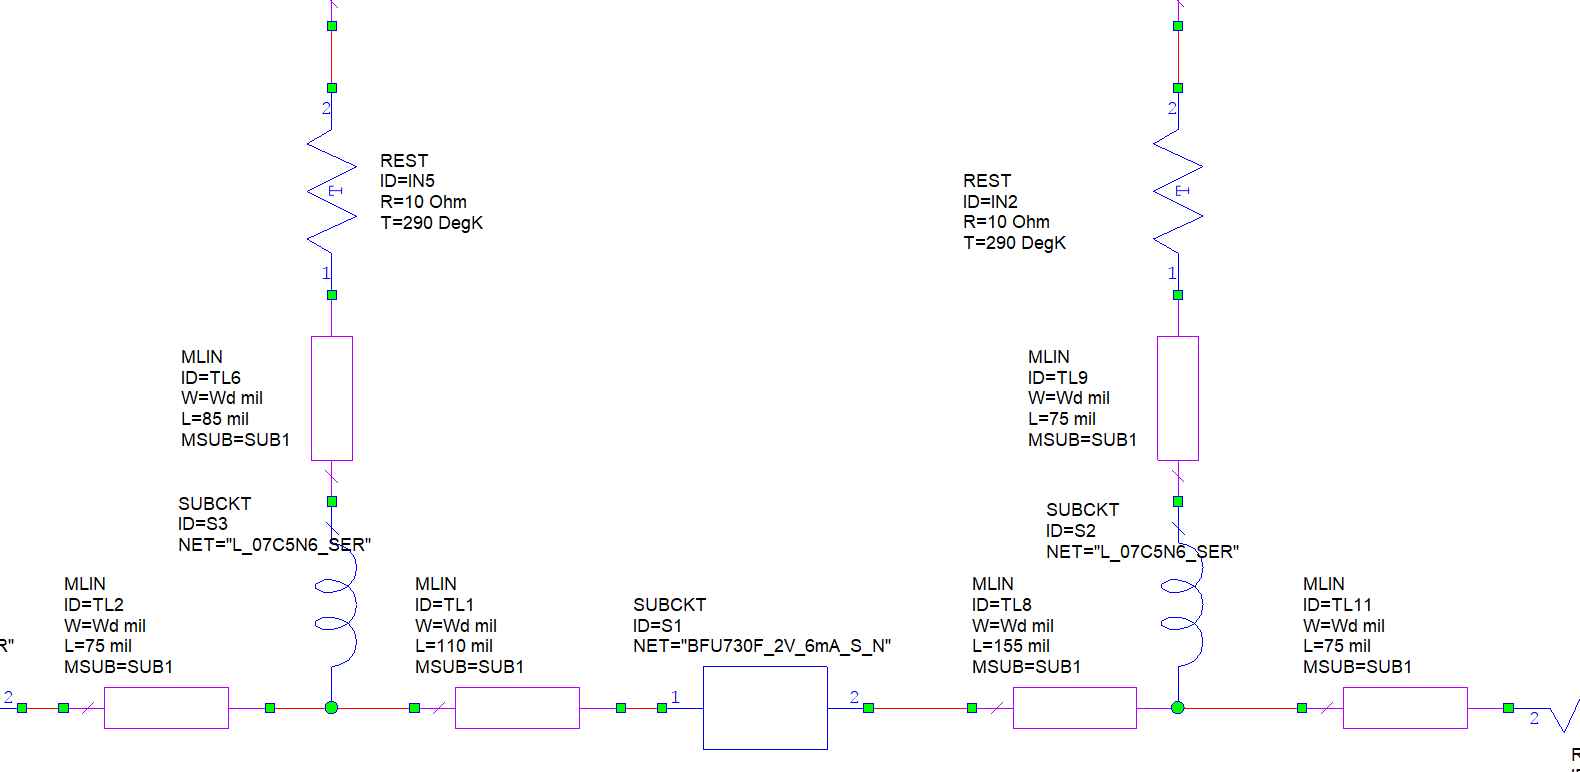
\includegraphics[scale=0.35]{LNA_net.png}
        \caption{Schematic showing the high impedance inductors used to stabilize the amplifier response. Small 10$\Omega$ resistors were also added in series to enhance stability.}
        \label{fig:LNAnet}
    \end{figure*}

    \begin{figure}[!htbp]
    \centering
    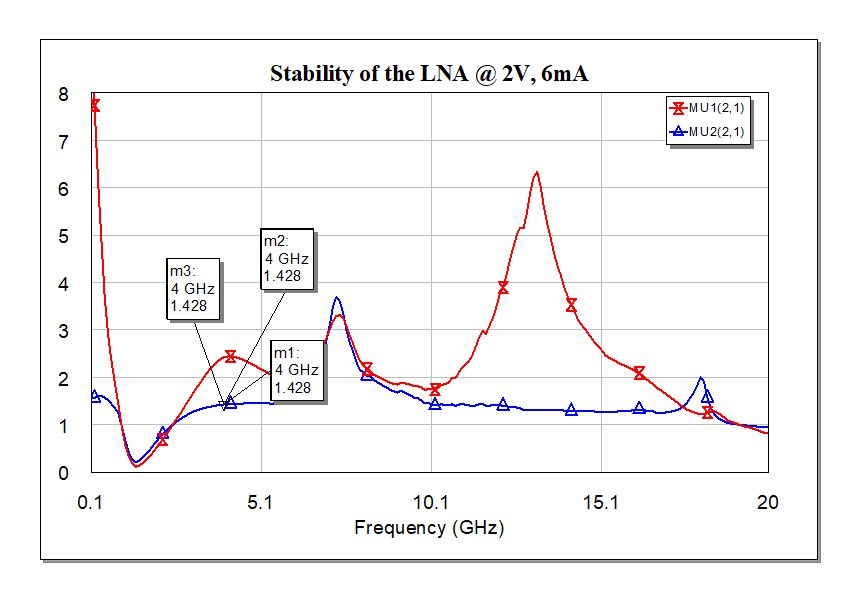
\includegraphics[scale=0.3]{stability.png}
    \caption{A plot of the stability parameters, $\mu_1, \mu_2$ of the network. We have good stability in region where either $\mu_1 > 1$ or $\mu_2 > 1$. }
    \label{fig:stability}
    \end{figure}

    \item Designed the input matching network, by choosing $\Gamma_s = \Gamma_{opt}$ as determined for our choice of bias and stability network for the amplifier. The network designed in MWO. And the schematic is shown in figure \ref{fig:inputnet}

    \begin{figure*}[!htbp]
    \centering
    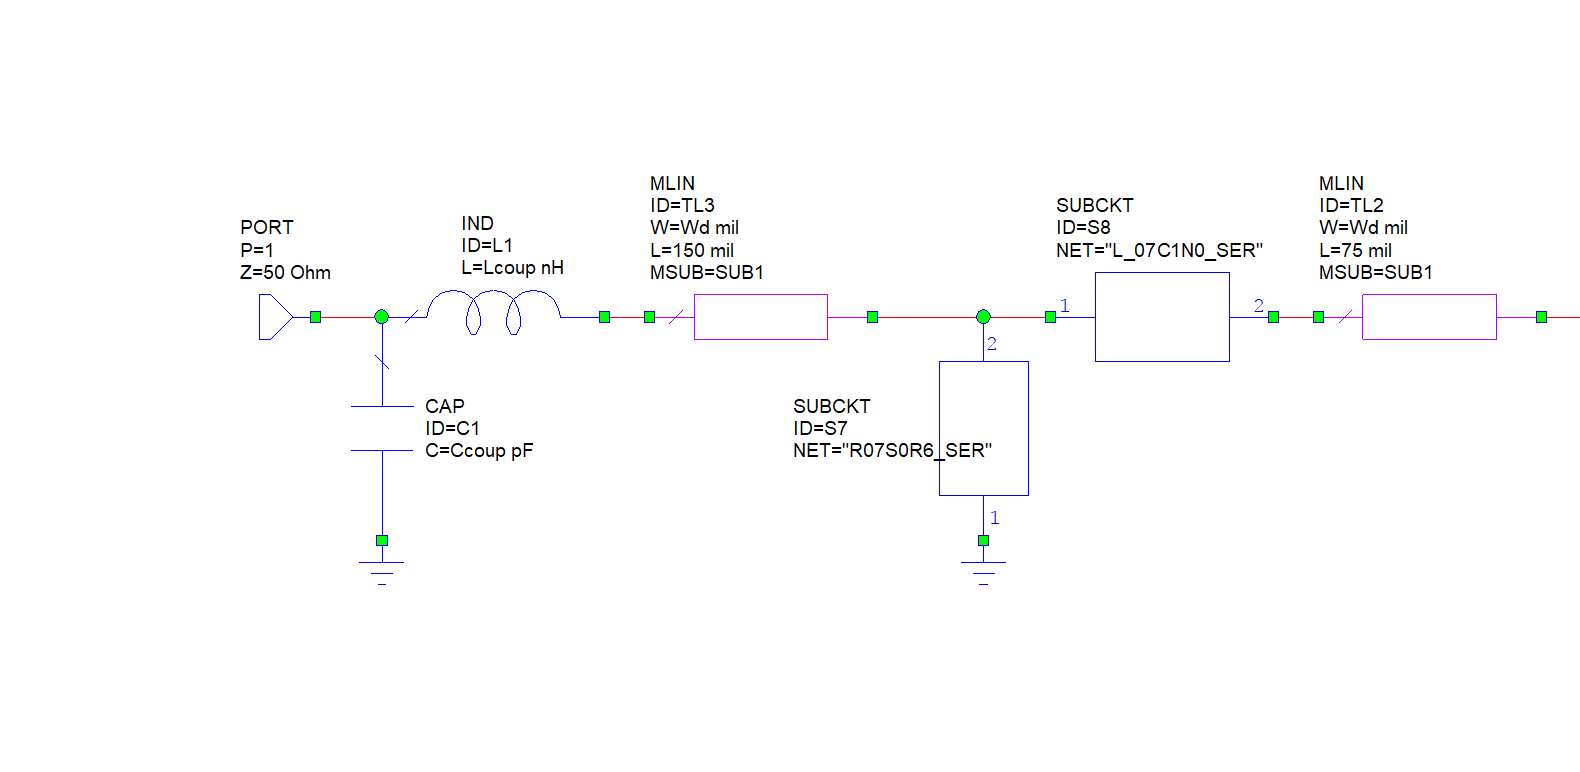
\includegraphics[scale=0.35]{input_net.png}
    \caption{Input matching network for the amplifier.}
    \label{fig:inputnet}
    \end{figure*}

    \item Designed the output matching network based on the value of $\Gamma_{in} = \Gamma_{opt}$ which fixes the value of $\Gamma_l$. The output matching network is shown in figure \ref{fig:outputnet}. The small resistor at the output of the amplifier was set to $30 \Omega$ for stability of the network at a slight cost to the gain of the system.

    \begin{figure*}[!htbp]
    \centering
    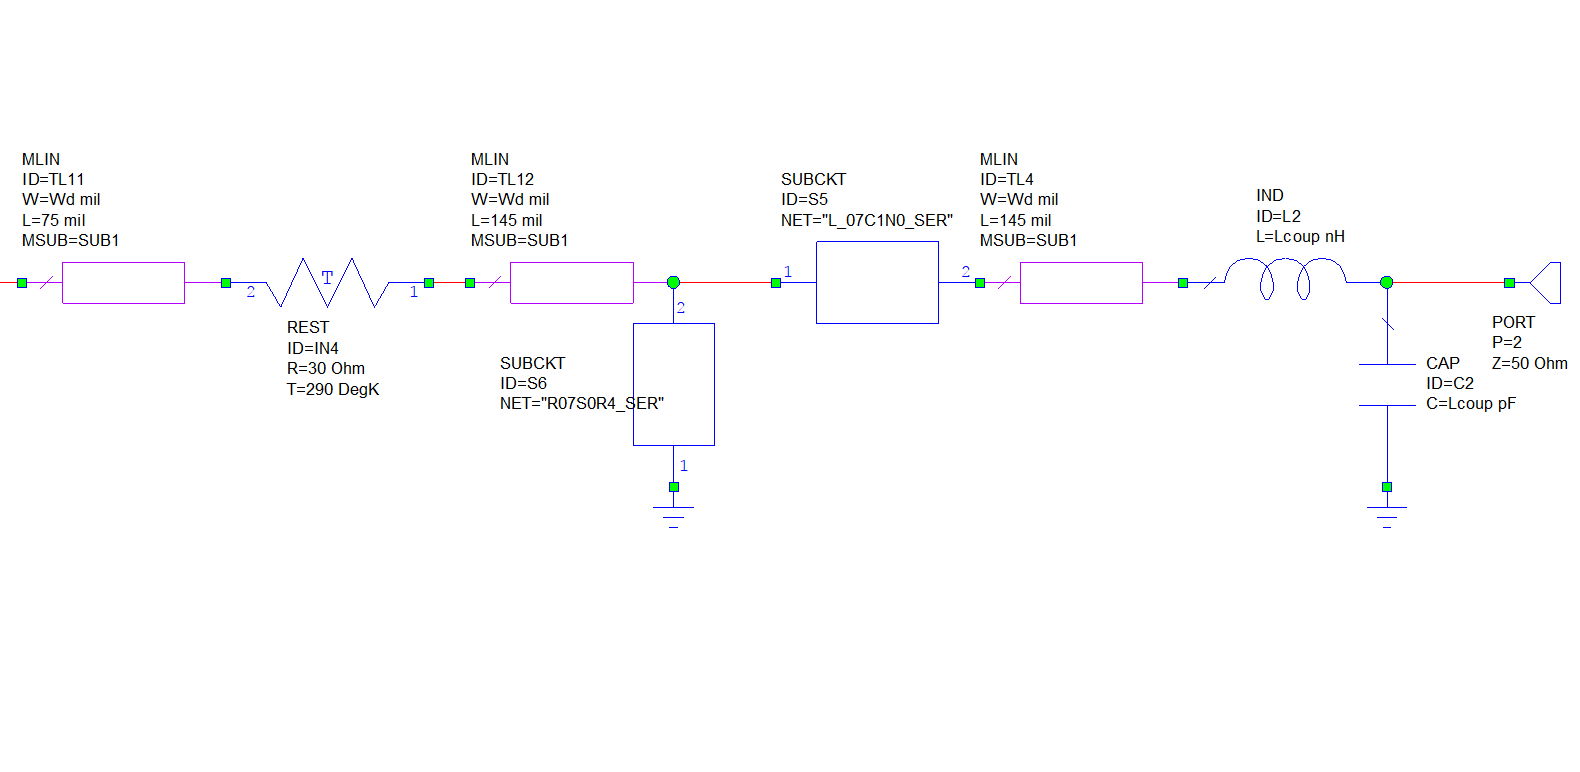
\includegraphics[scale=0.35]{output_net.png}
    \caption{Output matching network for the amplifier.}
    \label{fig:outputnet}
    \end{figure*}

    \item Design noise temperature $T_e = 58.35 K$ at 4 GHz. Only slightly above the minimum noise temperature for the choice of transistor.

\end{itemize}

\section*{Lab Testing}

\begin{itemize}
    \item populated the board with all the necessary capacitors, inductors, connectors and resistors as well as the BJT. Soldered all the components onto the board. Added a 10pF DC block to the RF input of the network because the Noise Figure Analyzer is not ac coupled. 

    \item Calibrated the VNA at -30.0 dBm input power and measured the S parameters of the amplifier circuit. Setup see figure \ref{fig:ampimg}. OVP at 2.50V and OCP at 0.01 A. See figure \ref{fig:ampSparams}.

    \begin{figure}[!htbp]
    \centering
    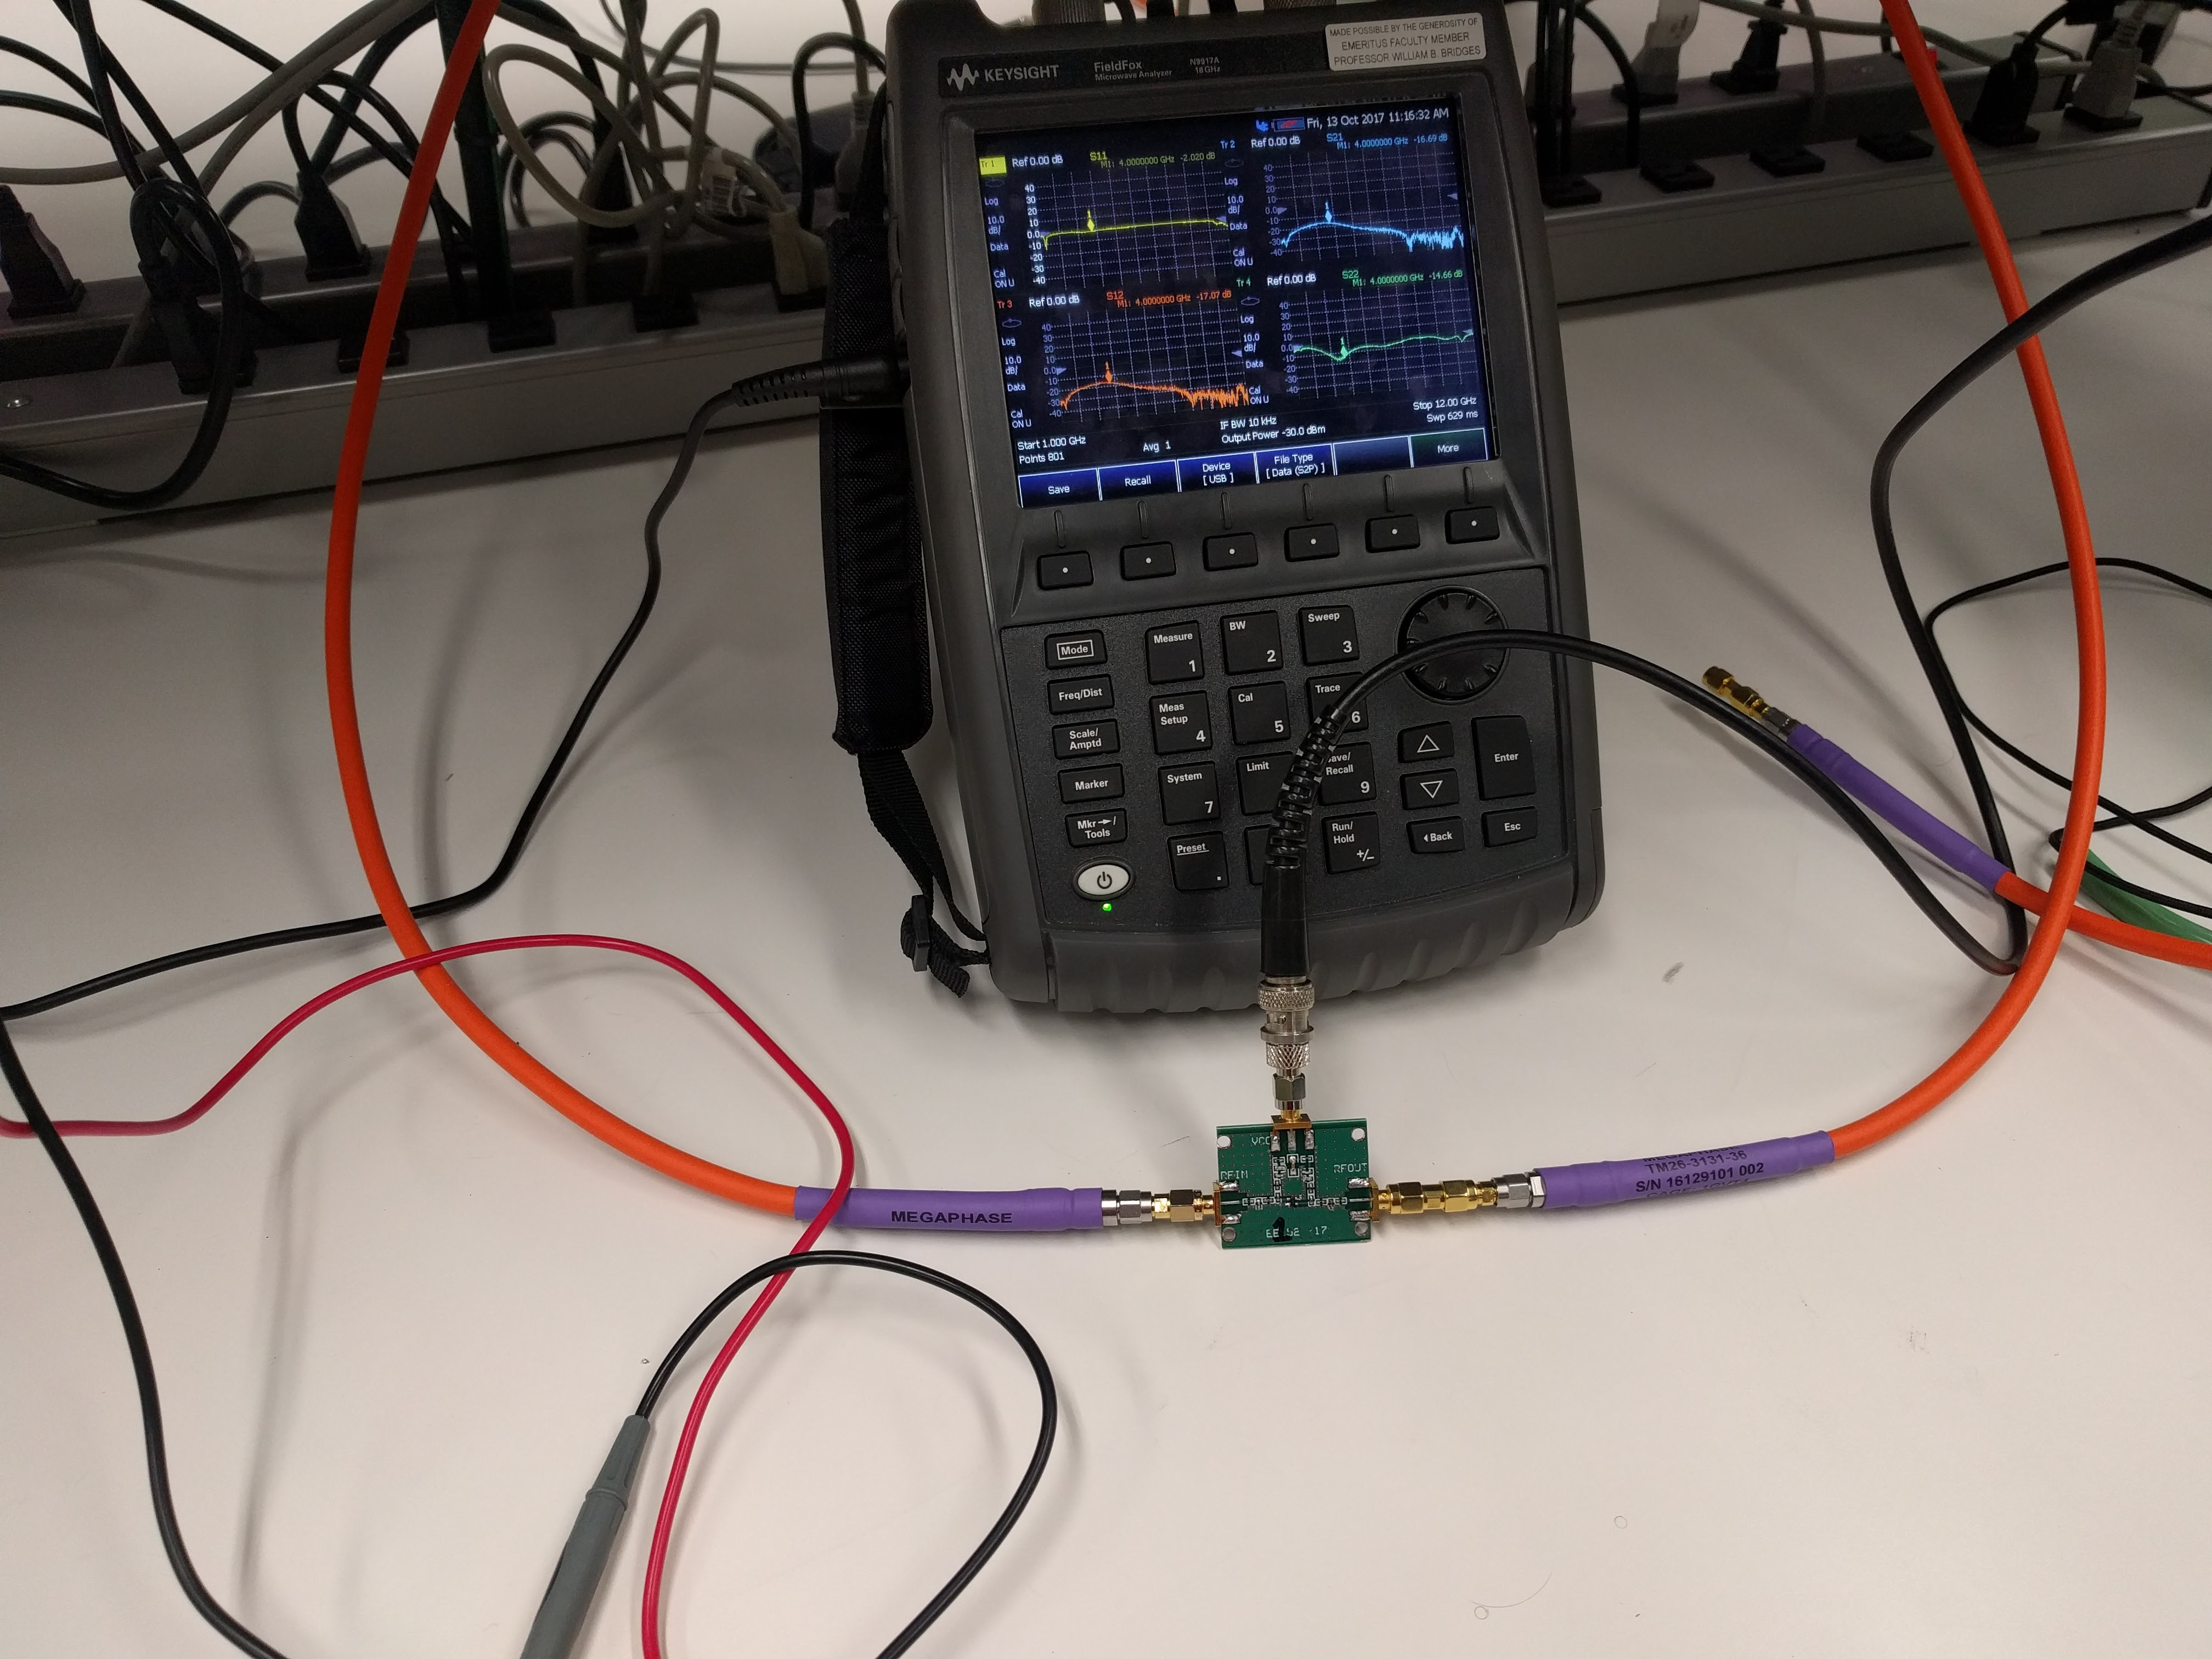
\includegraphics[scale=0.05]{LNA_1.jpg}
    \caption{FieldFox setup for S parameter measurements on the low noise amplifier.}
    \label{fig:ampimg}
    \end{figure}

    \begin{figure}[!htbp]
    \centering
    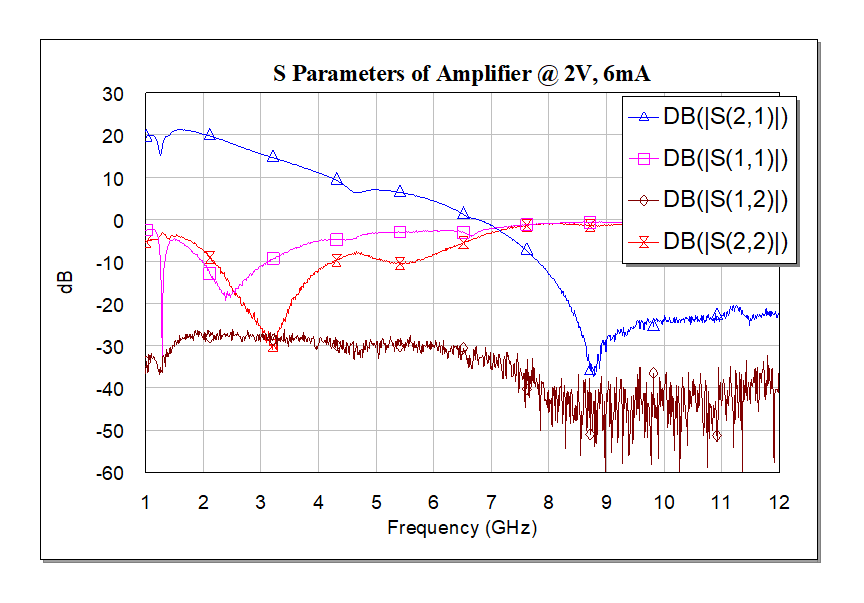
\includegraphics[scale=0.3]{amp_S_params.png}
    \caption{Measured S parameters of the amplifier at -30.0 dBm input power.}
    \label{fig:ampSparams}
    \end{figure}

    \item Recalibrated the VNA to a -5.0 dBm input power level for better measurements of the filter response. Setup see figure \ref{fig:filterimg}. Measured the S parameters of the filter. See figure \ref{fig:filterSparams}.

    \begin{figure}[!htbp]
    \centering
    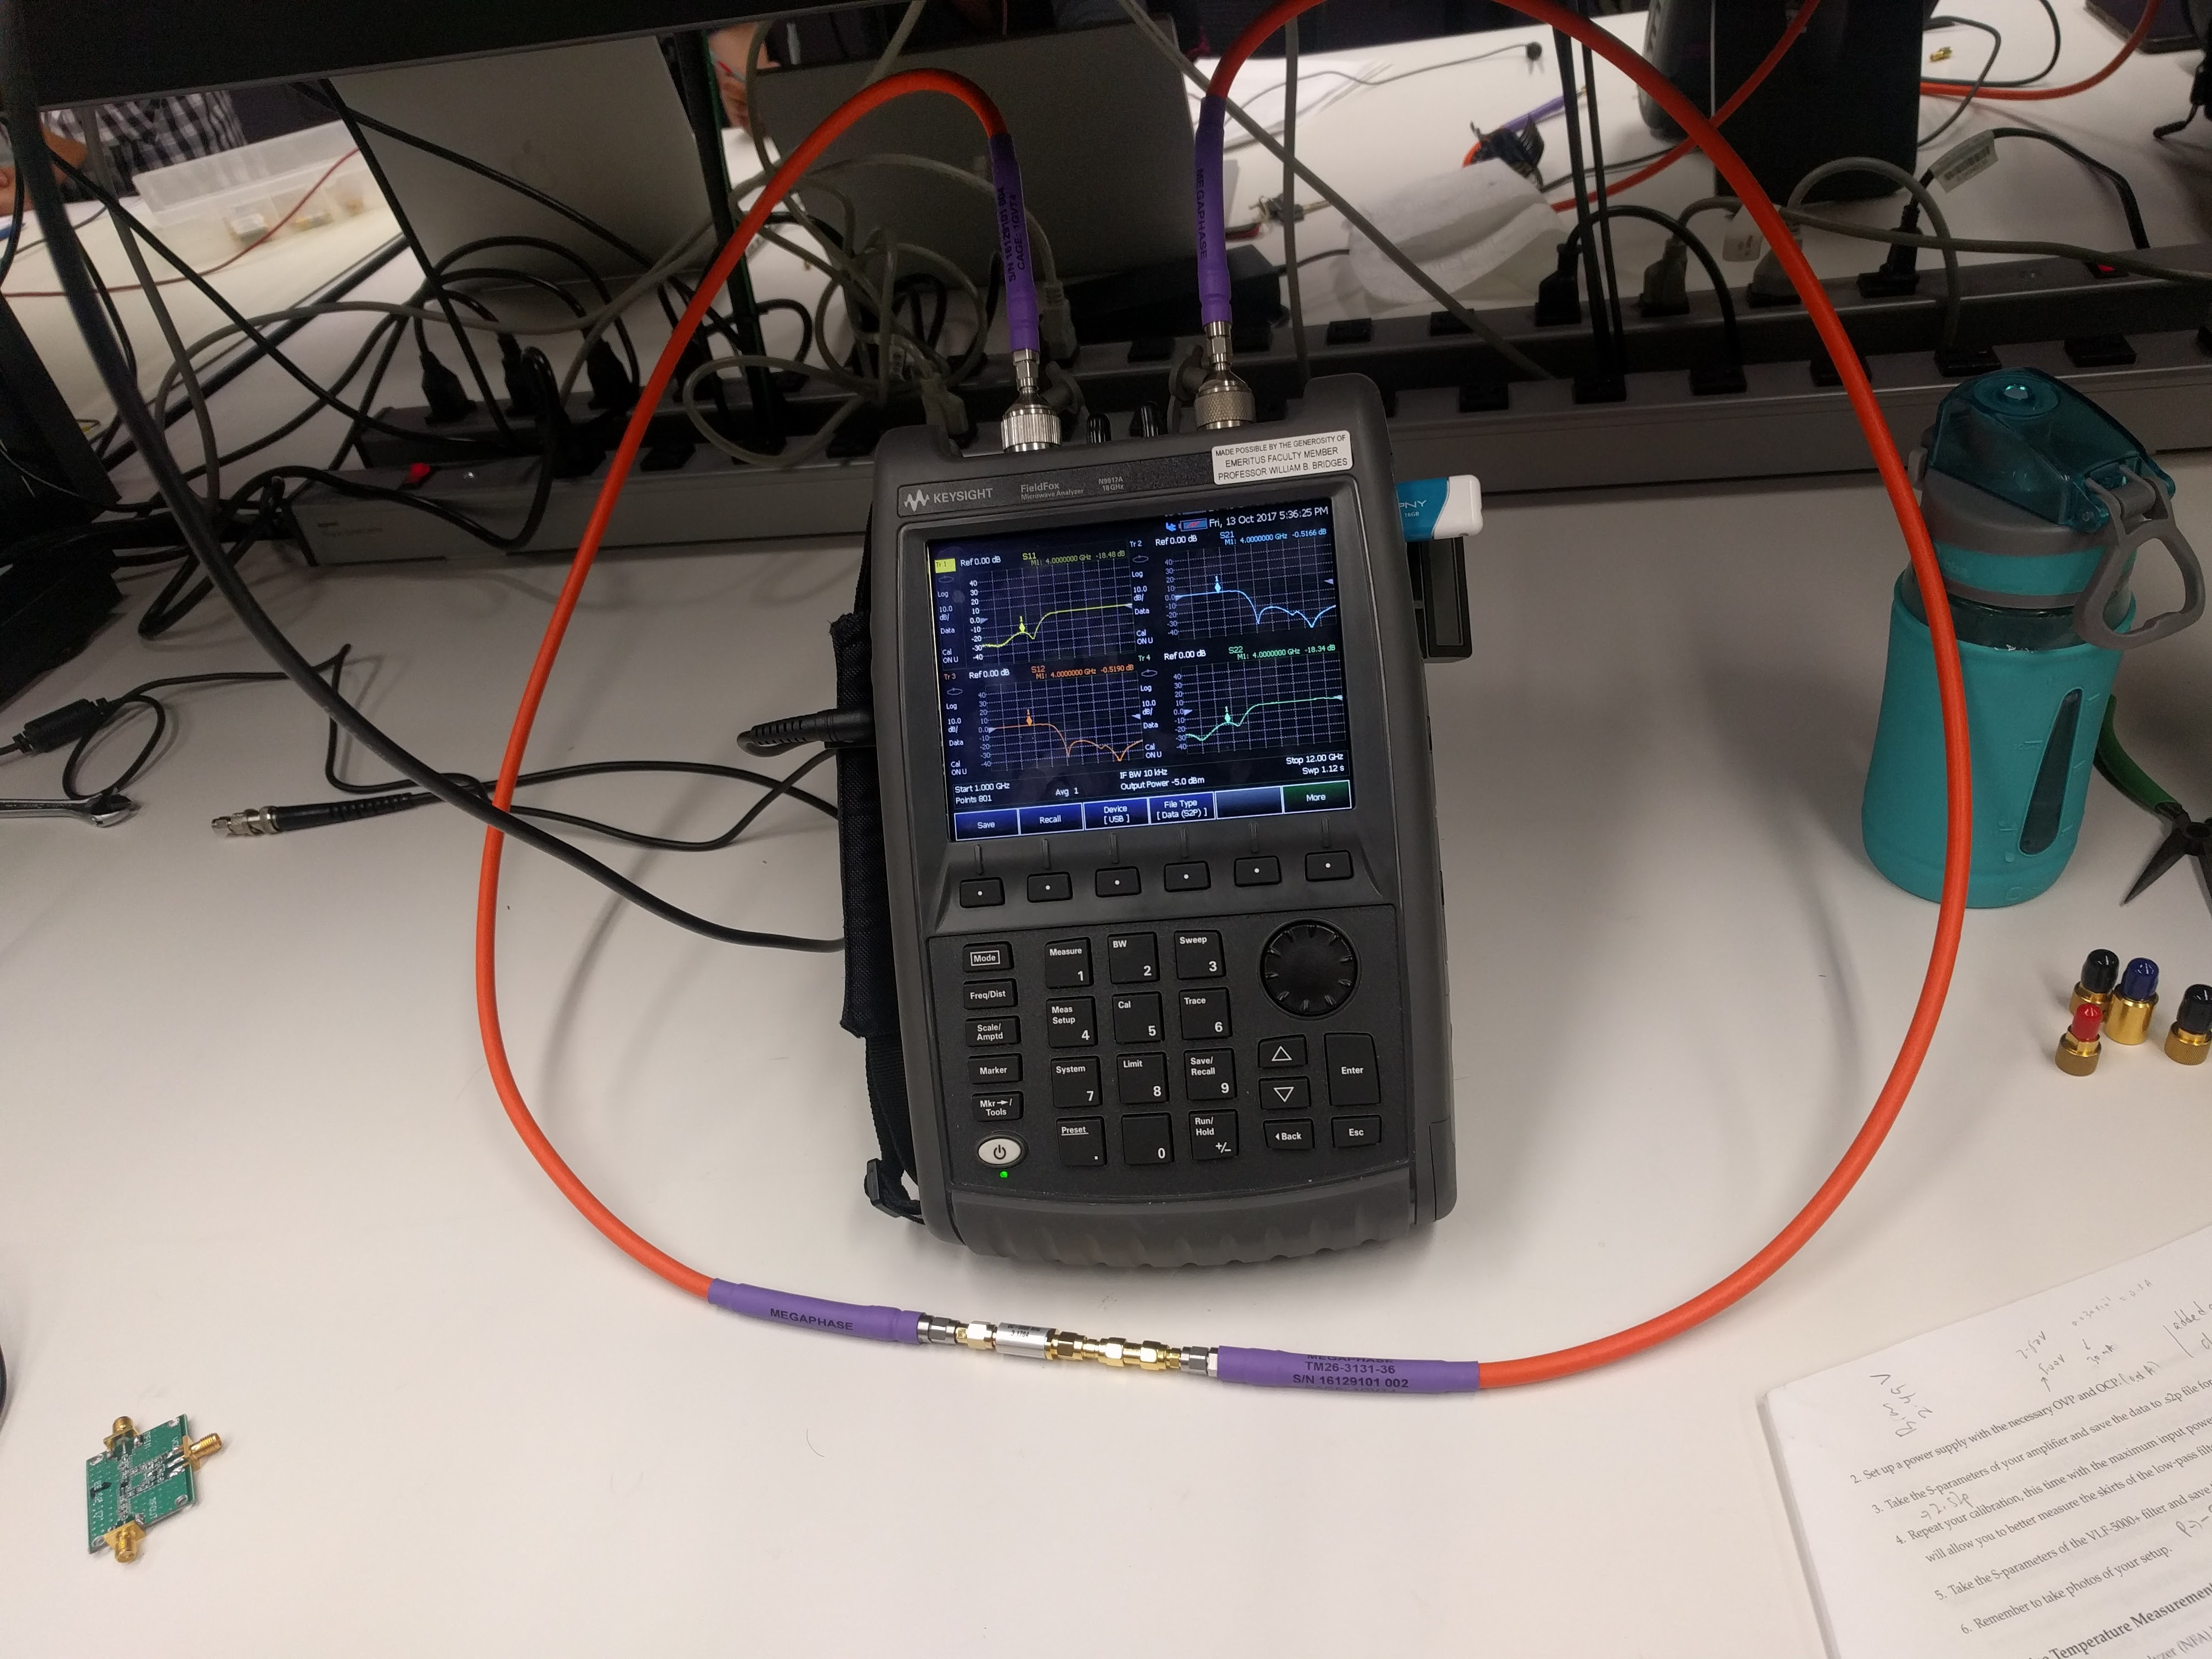
\includegraphics[scale=0.05]{Filter.jpg}
    \caption{Measurement setup for the S parameters of the Low Pass Filter.}
    \label{fig:filterimg}
    \end{figure}

    \begin{figure}[!htbp]
    \centering
    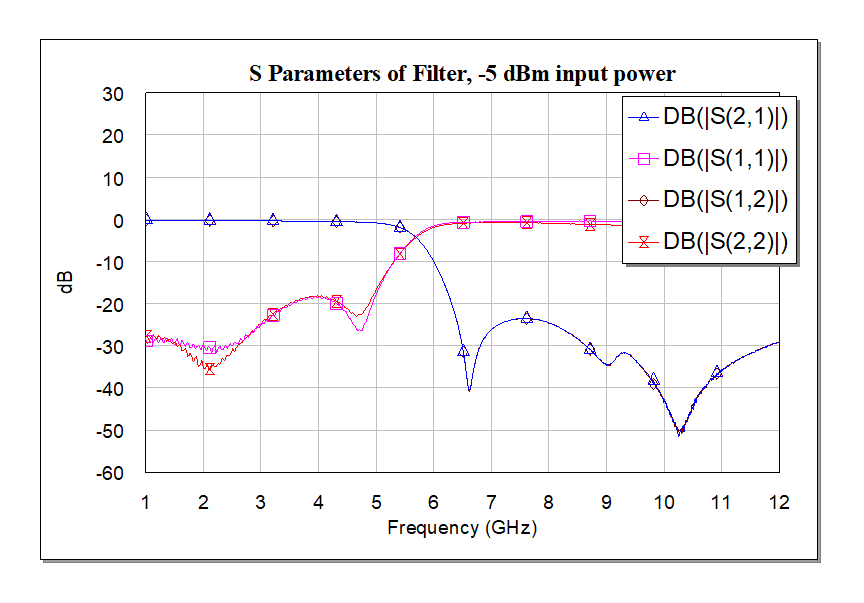
\includegraphics[scale=0.35]{filter_S_params.png}
    \caption{Measured S parameters of the filter at -5.0 dBm input power.}
    \label{fig:filterSparams}
    \end{figure}


\end{itemize}

\subsection{Noise Measurements}

\begin{itemize}
    \item for the Y factor measurements, used a Noise Figure Analyzer (NFA) calibrated to a room temperature (290 K) noise source.

    \item plugged the noise source to the input of the amplifier and the output port of the amplifier to the NFA. Same biasing at 2V and 6mA as shown in figure \ref{fig:ampnoiseimg}.

    \begin{figure}[!htbp]
    \centering
    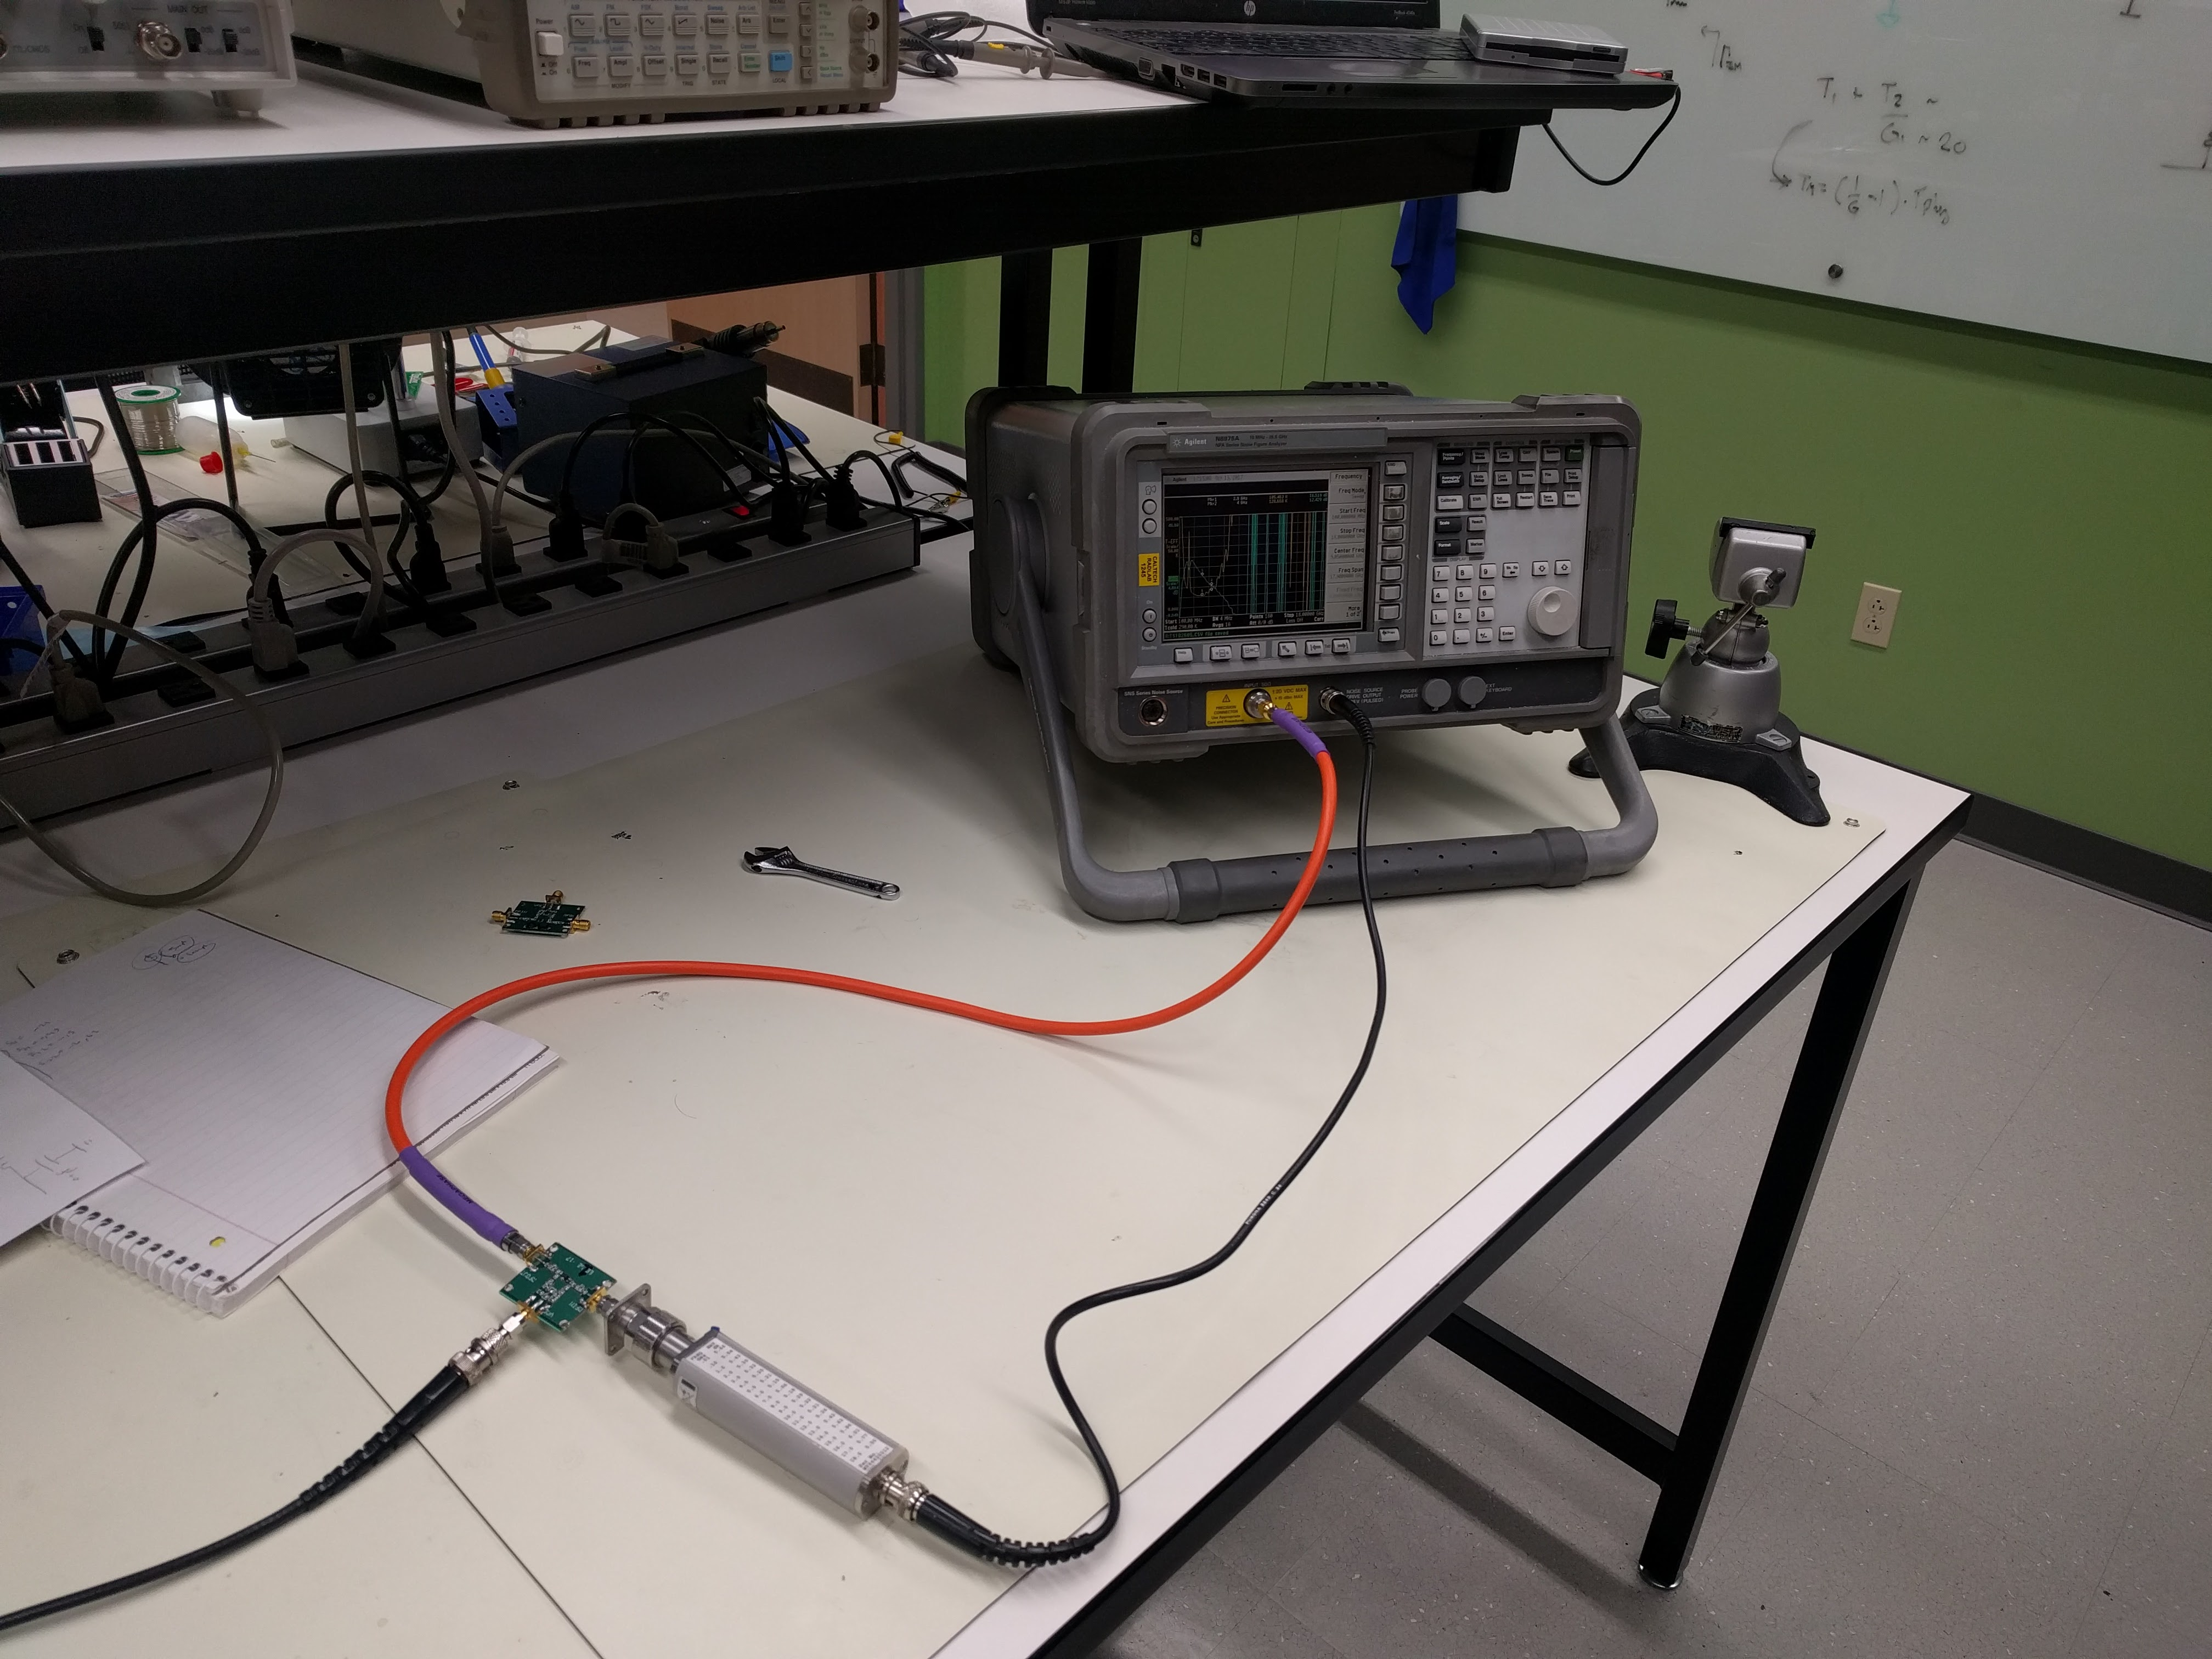
\includegraphics[scale=0.05]{LNA_Noise.jpg}
    \caption{Noise measurement setup using the NFA, noise source and the amplifier}
    \label{fig:ampnoiseimg}
    \end{figure}

    \item swept through frequency range twice and saved the noise and gain data. Effective temperature, $T_e = 128.668 K$, a factor of about 2.2 times higher than the expected noise levels. A plot of the equivalent input noise temperature, as simulated vs. measured shown in figure \ref{fig:amptempcomparison}.

    \begin{figure}[!htbp]
    \centering
    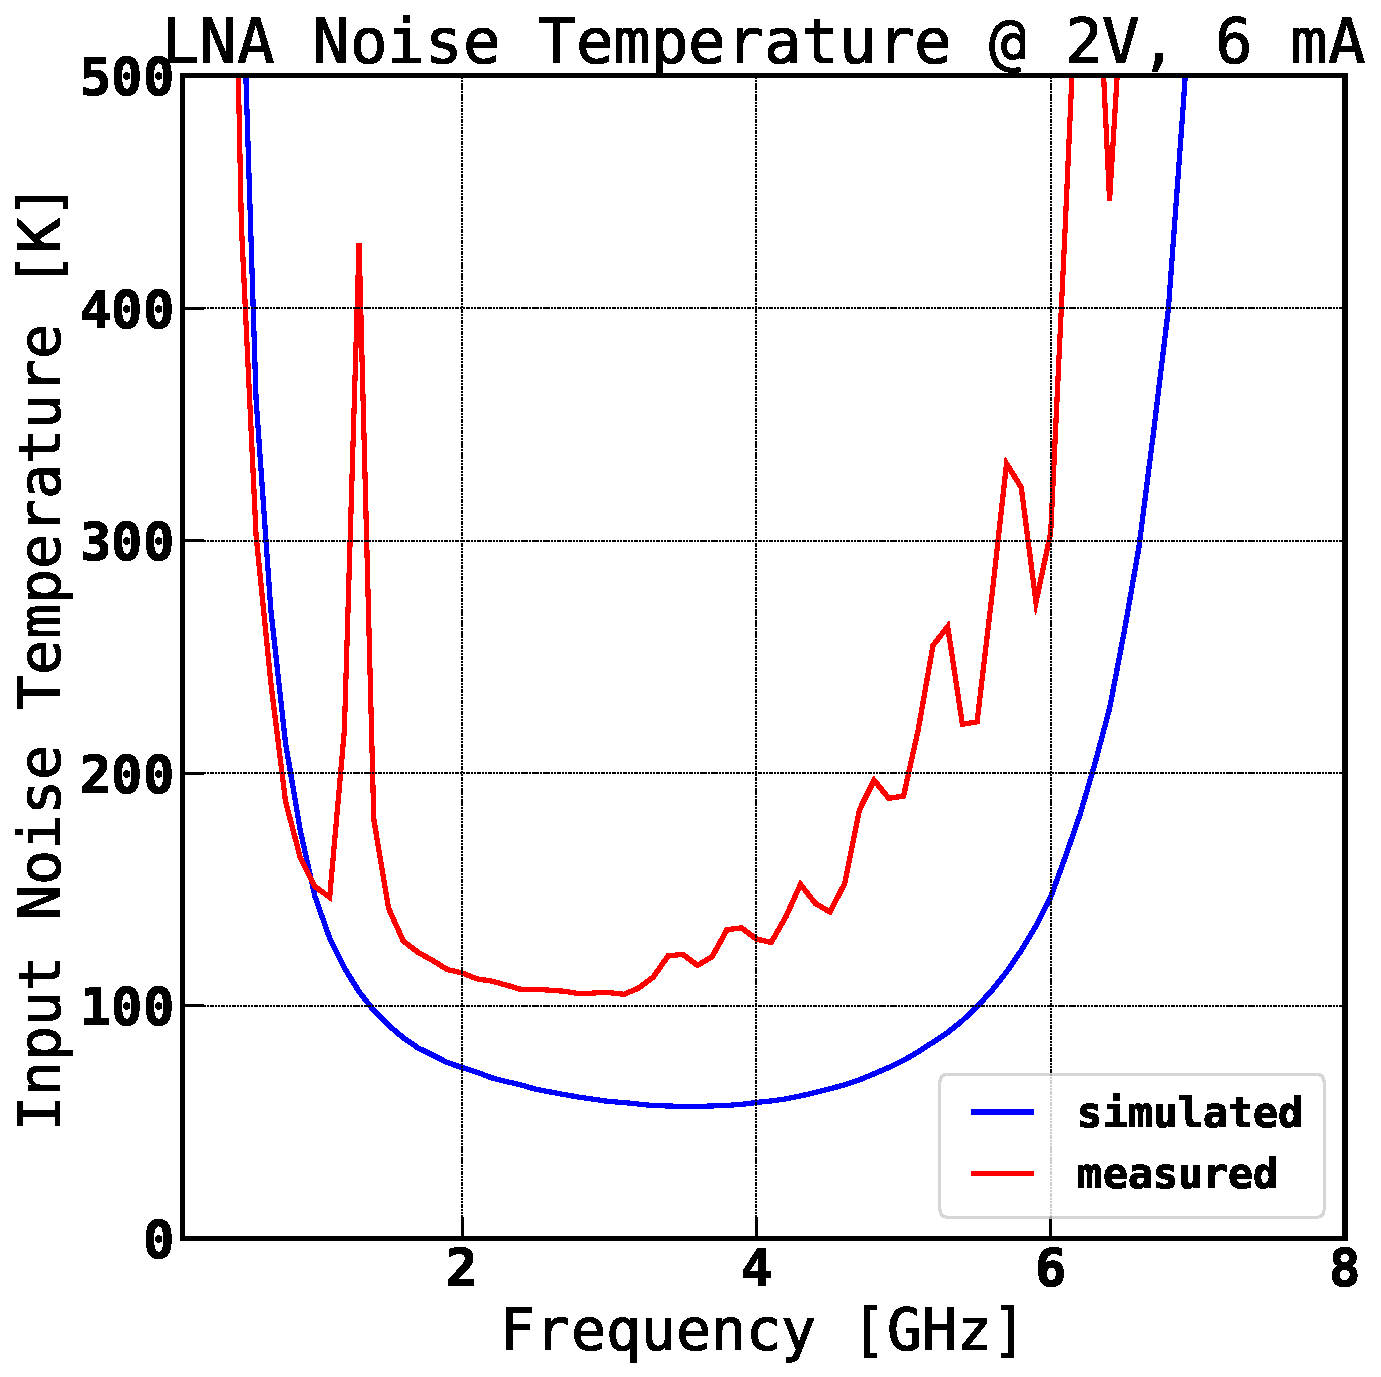
\includegraphics[scale=0.3]{LNA_noisetemp_comparison.pdf}
    \caption{A comparison of the measured vs. simulated noise performance of the amplifier. The high excess noise above 1 GHz is clearly visible.}
    \label{fig:amptempcomparison}
    \end{figure}

    \item Hooked up the low pass filter to the input of the amplifier and retook the measurements. As expected, the noise temperature was much higher at $T_e = 196.025 K$. With the filter at the output, the noise temperature was lower at $T_e = 128.81 K$. A comparison of the two measurements is shown in figure \ref{fig:filtertempcomparison}.

    \begin{figure}[!htbp]
    \centering
    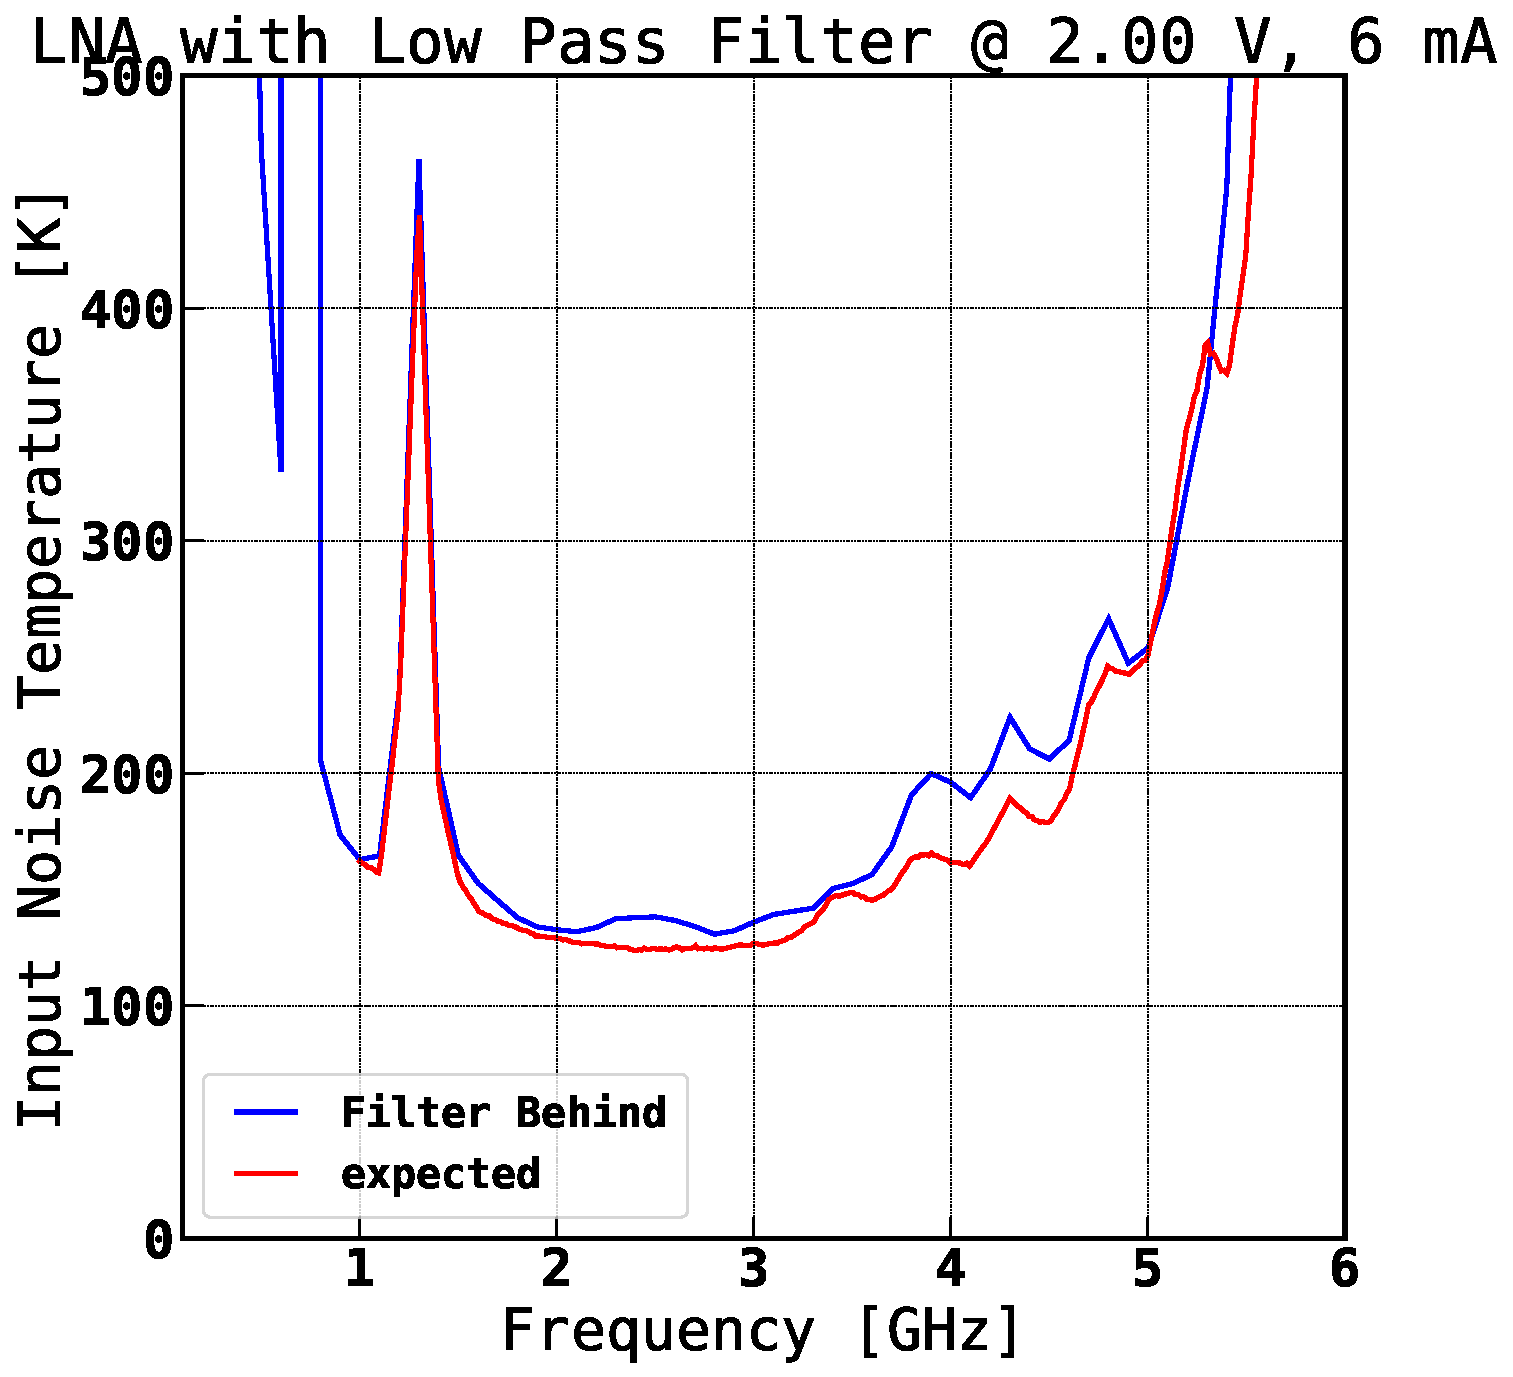
\includegraphics[scale=0.3]{Filter_noisetemp_comparison.pdf}
    \caption{A comparison of the noise performance of the amplifier with the filter at the input (behind) and filter at the output (ahead) of the LNA.}
    \label{fig:filtertempcomparison}
    \end{figure}

\end{itemize}

\section*{Analysis}

\begin{itemize}
    \item The simulated and measured noise temperature of the LNA showed strong deviations \ref{fig:amptempcomparison}. The shape of the noise temperature profile as a function of the frequency was the same, but elevated at higher frequencies. Given more time, I would have attempted to account for noise contributions from the passives in the network as well as from the power supply. Maybe something else but need ideas!!!

    \item The change in noise temperature between the filter at input and filter at output cases can be modelled well and with good accuracy. The Friis formula captures how to calculate the effective noise factor of a system based on the noise factors of the constituent subsystems. Given $F_i$ as the noise factor for the $i$th subsystem and $G_i$ as the gain of that subsystem, we can state the Friis formula as

    \begin{equation}
        F_{total} - 1 = (F_1 - 1) + \frac{F_2 - 1}{G_1} + \frac{F_3 - 1}{G_1 \times G_2} + \ldots.  
    \end{equation} 

    Specializing it for our case, we note that for the amplifier, $F - 1 = \frac{T_e}{T_0}$ where $T_e$ is the equivalent input noise temperature of the amplifier as measured and $T_0 = 290 K$. For the low pass filter, following the discussion in the introductory section \ref{sec:introduction}, the noise factor is given by the relation $F - 1 = L - 1$, where L is the attenuation of the filter ($L = 1/G$).

    For the filter at the input of the amplifier, then the total effective temperature is given by

    \begin{equation}
        T_{TOT, behind} = T_{LNA} + \frac{L - 1}{G_{LNA}} \times T_0.
    \end{equation}

    Using this equation, I have plotted a comparison between the measured and expected effective noise temperature as shown in figure \ref{fig:behindnoisetemp}
    
    \begin{figure}[!htbp]
    \centering
    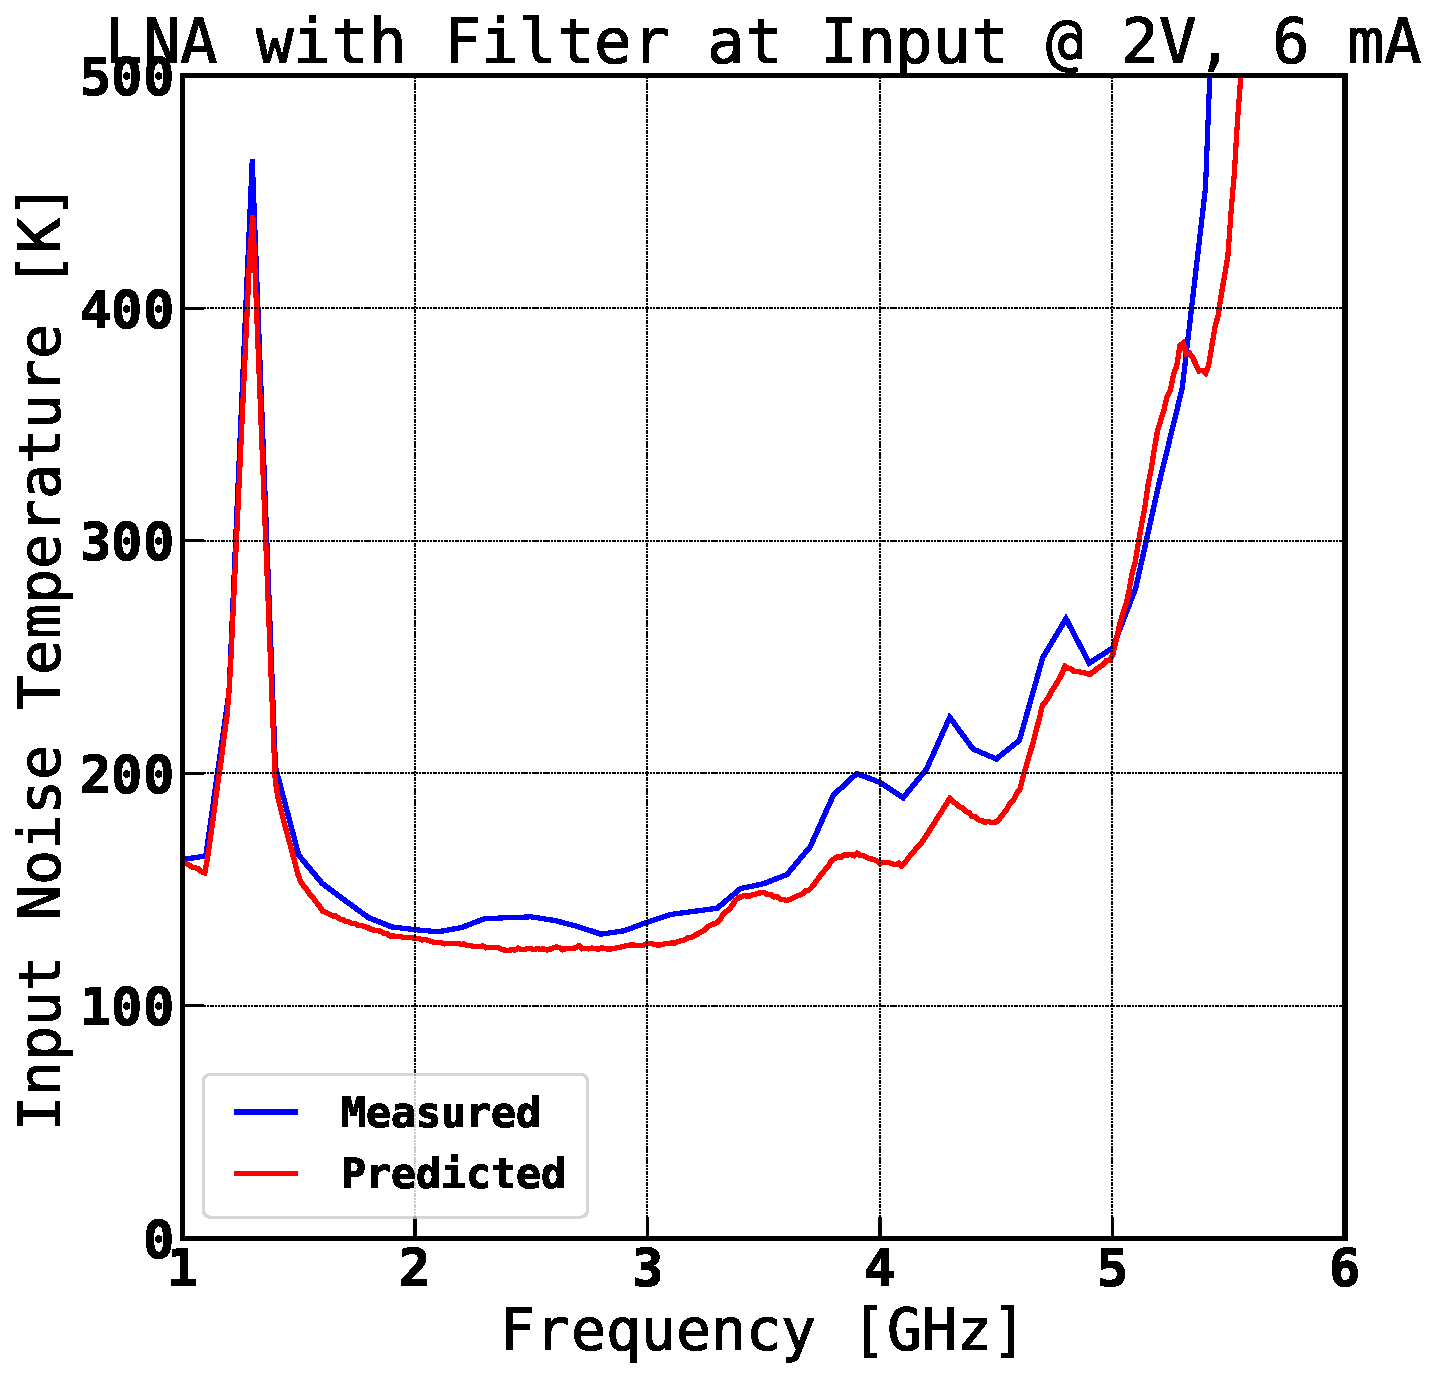
\includegraphics[scale=0.3]{Filter_behind_noisetemp.pdf}
    \caption{A comparison of expected and measured noise performance of the amplifier with the filter at the input (behind) of the LNA.}
    \label{fig:behindnoisetemp}
    \end{figure}

    On the other hand, when the filter is placed at the output of the amplifier, then the total effective temperature is given by

    \begin{equation}
        T_{TOT, ahead} = \left(L - 1 \right) \times T_0 + L \times T_{LNA}.
    \end{equation}

    Similarly, we can compare the predicted effective temperature from this equation with the actual measured performance as shown in figure \ref{fig:aheadnoisetemp}.
    \begin{figure}[!htbp]
    \centering
    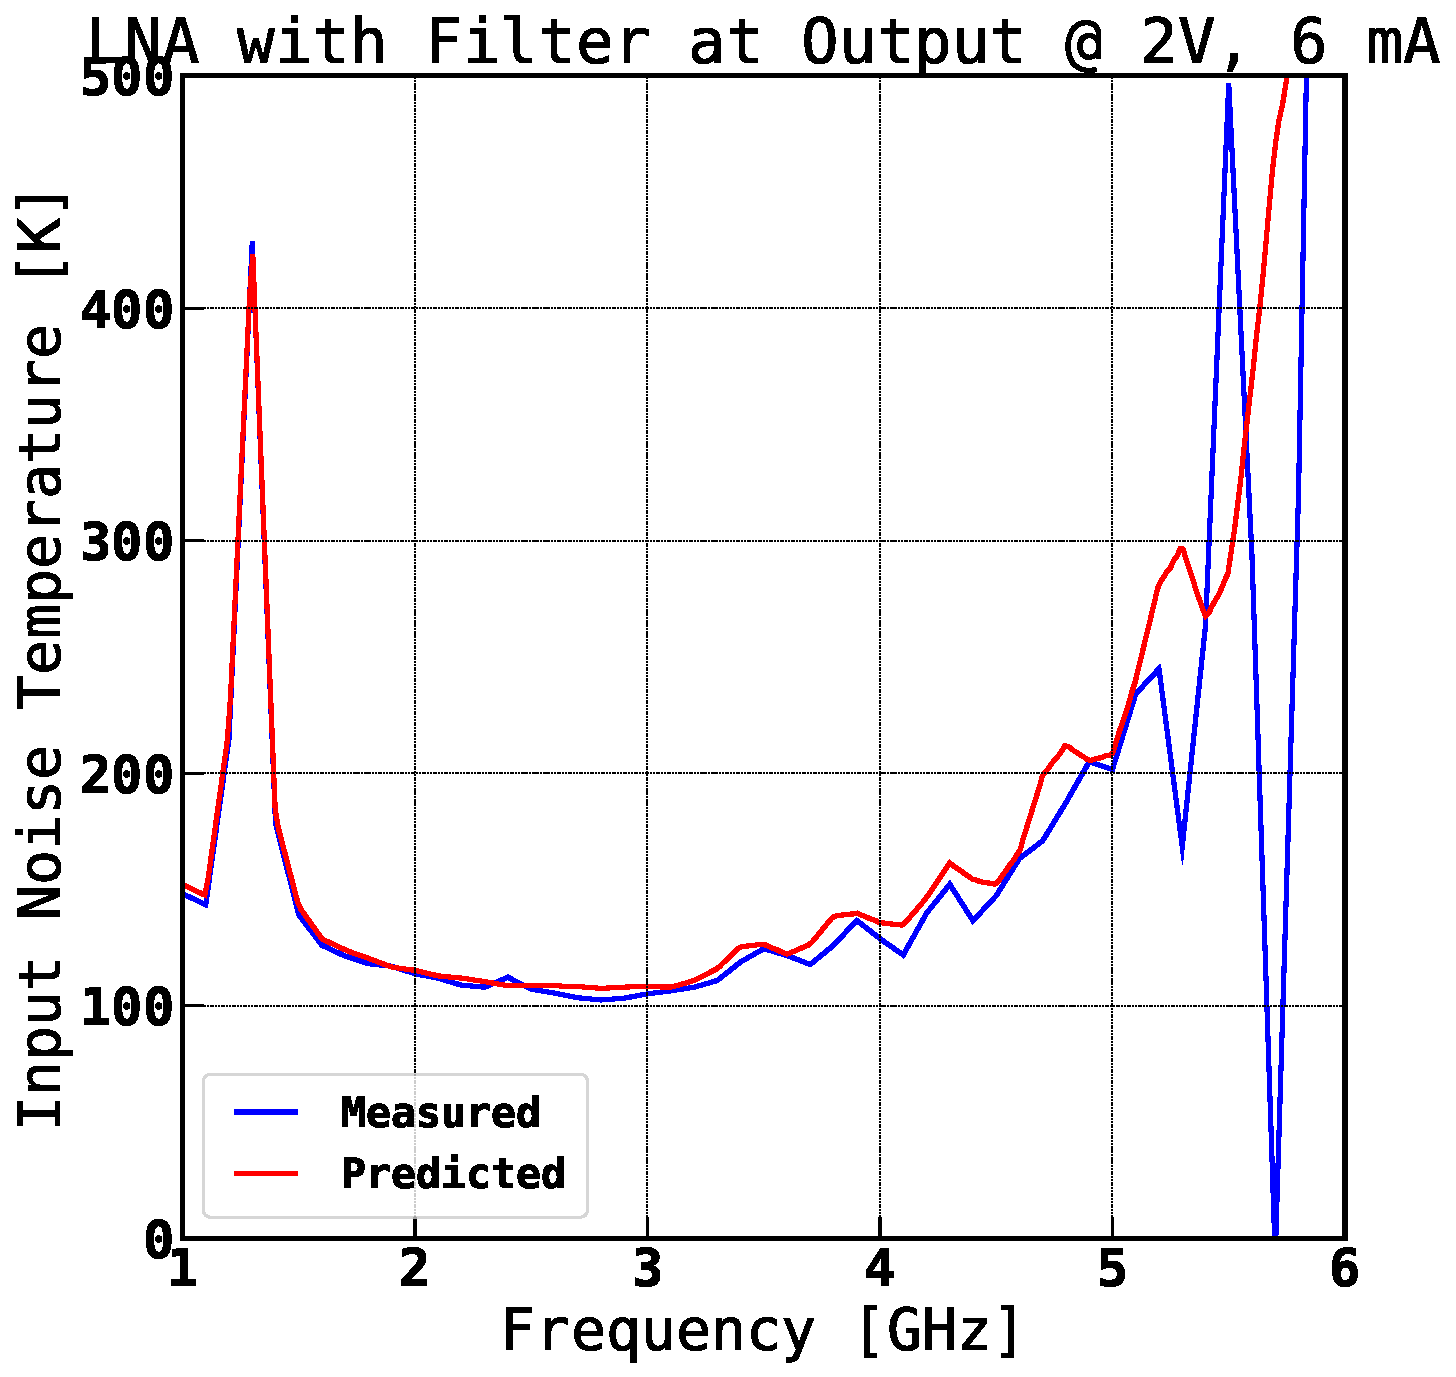
\includegraphics[scale=0.3]{Filter_ahead_noisetemp.pdf}
    \caption{A comparison of expected and measured noise performance of the amplifier with the filter at the output (ahead) of the LNA.}
    \label{fig:aheadnoisetemp}
    \end{figure}

    A comparison of these two equations, immediately shows why we have a higher effective temperature when the filter is at the output. Since the filter is a passive device, its gain is always less than 1 and as a result, $L > 1$. If the amplifier has a high enough gain, then the gain factor in the denominator makes that term very small and thus for the filter behind case, $T_{TOT} \approx T_{LNA}$. For the filter ahead case, we instead have $T_{TOT} \approx L \times T_{LNA}$ which would be bigger since L is greater than 1.


    \item Simulations of the amplifier circuit with the filter at the input show an expected equivalent temperature of 100.2 K up from about 60.86 K. This deviation is partly due to the mismatch at the input introduced by the filter. In the filter band, the filter has a very small reflection coefficient. Talk about this some more.

    \item Adding shunt capacitors and series inductors at the ports to model parasitics gives a slightly better match in the frequency range 1.5 - 4.5 GHz. In addition, slight changes to the values of the matching network help create a better match between simulation and measured behavior. However, a good match could not be found over the entire frequency range of interest. Improvements at low frequencies led to a much worse match at high frequencies. We can thus account well for the behavior close to the design frequency of 4 GHz but not at much higher frequencies. See \ref{fig:changedampsims}

    \begin{figure}[!htbp]
    \centering
    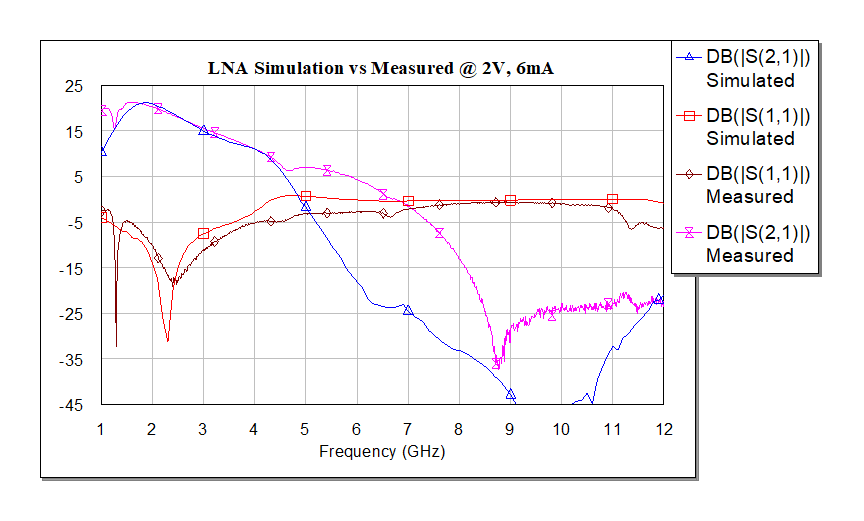
\includegraphics[scale=0.4]{LNA_simulated_measured.png}
    \caption{A comparison of expected and simulated amplifier response chosen to better match with the measured response.}
    \label{fig:changedampsims}
    \end{figure}

\end{itemize}

\section*{Conclusions}

This lab gave me good experience with the design considerations in making a good low noise amplifier. I have a better appreciation of the difficulties inherent in identifying all possible noise sources to try and achieve some desired noise specifications. There was also plenty of lab experience in soldering and hopefully the time put in now will pay off in future labs and projects. 
\end{document}